\section{The statistical lens: relevance, uncertainty, and the anti-ordinal
argument}\label{sec:stats}

\subsection{Why not a risk matrix}\label{sec:antiordinal}

The default instrument of enterprise risk is the ordinal matrix (likelihood
rows, impact columns, color-coded cells). Three independent literatures say not
to use it here. Cox showed that ordinal risk matrices can invert the true
ranking: under realistic distributions of independent likelihood and severity, a
matrix can systematically rate a more dangerous class as safer than a less
dangerous one \cite{cox2008}. Axelsson demonstrated the base-rate fallacy in
exactly our setting: intrusion-detection systems with excellent true-positive
rates are still useless at realistic attack base rates because false positives
dominate the arithmetic \cite{axelsson1999}. EPSS made the empirical version
official: CVSS severity scores are, in practice, weakly related to actual
exploitation probability---which is why EPSS exists as a probability instrument
built from exploitation telemetry (median score ${\sim}0.007$, 95th percentile
${\sim}0.10$, only ${\sim}1.2\%$ of CVEs above 0.5) \cite{epss-first,epss-paper}.
The common thread: \emph{rank by calibrated quantity, not by bucket}. Our
relevance model follows EPSS's logic---probability $\times$ impact with an
explicit uncertainty treatment---and FAIR adds the
accounting layer for when monetary terms are needed \cite{fair}.

\subsection{Every rate carries an interval (Wilson)}\label{sec:wilson}

For a measured proportion $\hat p = x/n$, the Wilson score interval is
\begin{equation}
\hat p \pm \frac{z}{1+z^2/n}\sqrt{\frac{\hat p(1-\hat p)}{n}+\frac{z^2}{4n^2}},
\qquad z = 1.96\ \text{(95\%)},
\label{eq:wilson}
\end{equation}
whose center is the shrunk estimate
$\frac{\hat p + z^2/2n}{1+z^2/n}$. Unlike the Wald interval it stays inside
$[0,1]$ at small $n$ and near the boundaries---exactly where red-team numbers
live. Table~\ref{tab:wilson} shows the worked cells this paper cites.

\begin{table}[htbp]
\centering\small
\caption{Wilson 95\% intervals for the paper's worked cells (computed by
\texttt{figures.py}; Eq.~\ref{eq:wilson}).}\label{tab:wilson}
\begin{tabular}{l r r r}
\toprule
Cell & $x/n$ & $\hat p$ & 95\% CI \\
\midrule
Undefended pool (pooled, Sec.~\ref{sec:pooling}) & 683/2312 & 0.295 & [0.277, 0.314] \\
Defended pool (pooled) & 93/1258 & 0.074 & [0.061, 0.090] \\
AgentDojo-style undefended cell & 79/229 & 0.345 & [0.286, 0.409] \\
Defended cell (tool firewall) & 17/219 & 0.078 & [0.049, 0.121] \\
Multilingual EN cell & 156/200 & 0.780 & [0.718, 0.832] \\
Multilingual low-resource cell & 162/200 & 0.810 & [0.750, 0.858] \\
Wildcard small cell & 3/20 & 0.150 & [0.052, 0.360] \\
\bottomrule
\end{tabular}
\end{table}

The small cell is the teaching row: a naive reading says ``15\%''; the interval
says ``somewhere between 5\% and 36\%''---which is the difference between a
dashboard and evidence.

\subsection{``We saw zero'' is not ``it is safe'' (rule of three)}\label{sec:rule3}

After $n$ trials with zero events, the 95\% upper bound on the true rate is
$1-0.05^{1/n} \approx 3/n$. Table~\ref{tab:rule3} is the planning ladder: with a
typical benchmark cell budget (10--20 attempts), a clean sweep only bounds the
rate at 0.14--0.26; bounds that matter need hundreds to thousands of attempts.

\begin{table}[htbp]
\centering\small
\caption{Zero-event upper bounds. ``Typical cell budget'' rows show what most
published cells can actually claim.}\label{tab:rule3}
\begin{tabular}{r l}
\toprule
$n$ trials, zero events & 95\% upper bound on rate \\
\midrule
10 & 0.259 \quad (typical manual suite) \\
20 & 0.139 \quad (typical cell budget) \\
30 & 0.095 \\
60 & 0.049 \\
300 & 0.010 \\
3000 & 0.001 \\
\bottomrule
\end{tabular}
\end{table}

\subsection{Pooling heterogeneous studies (Beta--Binomial)}\label{sec:pooling}

Merging all undefended rows of Table~\ref{tab:asr} into one binomial sample would
pretend studies are exchangeable---they are not (different targets, guards,
judges). Instead, each study $(x_i, n_i)$ gets a Beta($1,1$) posterior with mean
$(x_i{+}1)/(n_i{+}2)$ and sd $\sqrt{m(1-m)/(n_i{+}3)}$, and the pooled estimate
is the inverse-variance weighted combination. Our two pools:
\begin{align}
\text{undefended:}\quad & \mathbb{E}[p] = 0.296,\ \text{sd} = 0.010,\\
\text{defended:}\quad   & \mathbb{E}[p] = 0.075,\ \text{sd} = 0.007,
\end{align}
a defense ratio of $3.96\times$. Two honest readings: defenses \emph{work} ---
a four-fold cut is not nothing; and defenses \emph{do not finish}---a 7.5\%
residual rate across a large attack population is not a rounding error (the
at-least-one arithmetic of Section~\ref{sec:model} makes that explicit).

\subsection{Retry inflation and the resampling null}\label{sec:retry}

A harness that retries until success converts a per-attempt rate $p$ into a
per-session rate $1-(1-p)^k$. At PAIR-like economics ($p=0.03$, $k=20$ queries),
the session rate is 0.456 while the honest per-attempt number is 0.03---a
$15\times$ amplification produced entirely by patience. Our statistical layer
provides both directions (\texttt{session\_rate}, \texttt{per\_attempt}) and a
\texttt{resampling\_null} test: given per-attempt outcomes and $k$ retries per
session, it computes what exchangeable luck would produce and flags when the
observed session rate falls outside that band---the signature of success
clustering (adaptation, or a defender wearing down). A cell that cannot state
its retry policy has not yet earned its rate.

\subsection{Reliability across runs: pass$^k$}\label{sec:passk}

tau-bench's pass$^k$---the probability that a task passes on \emph{all} of $k$
independent runs---collapses brutally in practice (below 25\% at $k=8$ for
strong agents \cite{taubench}). Our \texttt{pass\_hat\_k} estimator bootstraps
completed runs into groups of $k$; the interval it returns is the honest price
of claiming ``our agent does $X$'' rather than ``did $X$ once''.

\subsection{The relevance model}\label{sec:model}

Each class $w$ gets
\begin{equation}
R(w) = P(w)\cdot I(w)\cdot \bigl(1-D(w)\bigr),
\label{eq:model}
\end{equation}
where $P$ is the elicited prior that the class materializes against a
defended-but-imperfect production stack, $I\in[1,5]$ is operator impact, and
$D\in[0,1]$ is defendedness measured by auditing our own code (what actually
blocks, detects, or contains the class today). The anchoring rule is explicit
and per-class (Table~\ref{tab:matrix}): prefer the best-documented
\emph{defended} measurement available (W1 anchors on the defended AgentDojo
residual); where the literature offers no defended anchor for the class (the
$^{\dagger}$ rows: W5's PoisonedRAG 90\%, W2's adaptive 100\%, W3, W13, W11),
the \emph{undefended} figure is used and the row is marked---those priors are
upper-bound anchors relative to the defended ones, and that asymmetry should be
carried when comparing rows. $R$ is a \emph{ranking
statistic}: we use it to order work, never as a probability statement about a
specific future event---the anti-ordinal argument of Section~\ref{sec:antiordinal}
applies to our own number with equal force. One further honesty note. Because
$P$ is elicited from published anchors and $D$ is an audit of our own code, the
ranking is a \emph{hypothesis about where the next hour of testing should
go}---an input to a work queue, not an evidence-fitted output. Its
falsification route is the acceptance tests of Section~\ref{sec:gaps}: a class
that resists a full campaign at its stated budget had its prior set wrong, and
the prior is updated. That loop---elicit, test, update---is the mechanism; a
ranking frozen at elicitation time would be exactly the stale ordinal
instrument Section~\ref{sec:antiordinal} warned against.

\paragraph{How many classes land at once.} With priors $\{P_w\}$, the expected
number of material classes per engagement is $\sum_w P_w = 5.35$ of fourteen.
The quantity $1-\prod_w (1-P_w) \approx 0.9994$ is the probability that at
least one class materializes \emph{computed under an independence assumption}---it is not the union bound (the Bonferroni union bound here is only
$\Pr[\exists\,w] \le \min(1,\textstyle\sum_w P_w)$, vacuous as a probability),
and independence is itself doubtful: classes share root causes (W1 injections
seed W3 cascades; W7 retry dynamics inflate every measured rate), and positive
correlation pushes the true at-least-one probability \emph{below} the
independence figure. The arithmetic is robust in exactly the direction the plan
needs: with every prior halved, the independence figure still reads $0.952$.
So the honest claim is not a calibrated joint probability---it is that several
classes land per engagement, which is what justifies breadth-first before
depth-first testing.

\paragraph{Sensitivity.} The procedure is stated, not asserted. Each Monte
Carlo draw redraws every prior $P_w$ and every defendedness $D_w$
independently, adding $\mathrm{Uniform}(-0.10,+0.10)$ (clipped to
$[0.02,0.95]$ for $P$, $[0,1]$ for $D$), holds $I$ fixed (a rubric, not a
measurement), recomputes the full ranking, and repeats $10{,}000$ times
(seed 42; \texttt{figures.py} prints the counts). Results: W5 holds rank 1 in
$100\%$ of draws and $\{$W5, W2$\}$ hold the top two positions as a set in
$100\%$---the head of the ranking is not an artifact of the elicited priors.
The middle is a genuine cluster: ranks 3--10 survive as a \emph{set} in only
$28.6\%$ of draws, because their $R$ values span just $0.74$--$1.33$ (W12 and
W6 are both inside the top 4 in only $30.4\%$ of draws). The deterministic
shifts agree: $+0.10$ on every $P$ leaves the top three unchanged; $-0.10$
swaps W6/W12 at rank 3. The plan therefore treats ranks 1--2 as firm and ranks
3--10 as one bundle with intra-bundle priority, not as fourteen crisp
positions. Figure~\ref{fig:relevance} renders the full ranking with lens
coloring.

\begin{figure}[t]
\centering
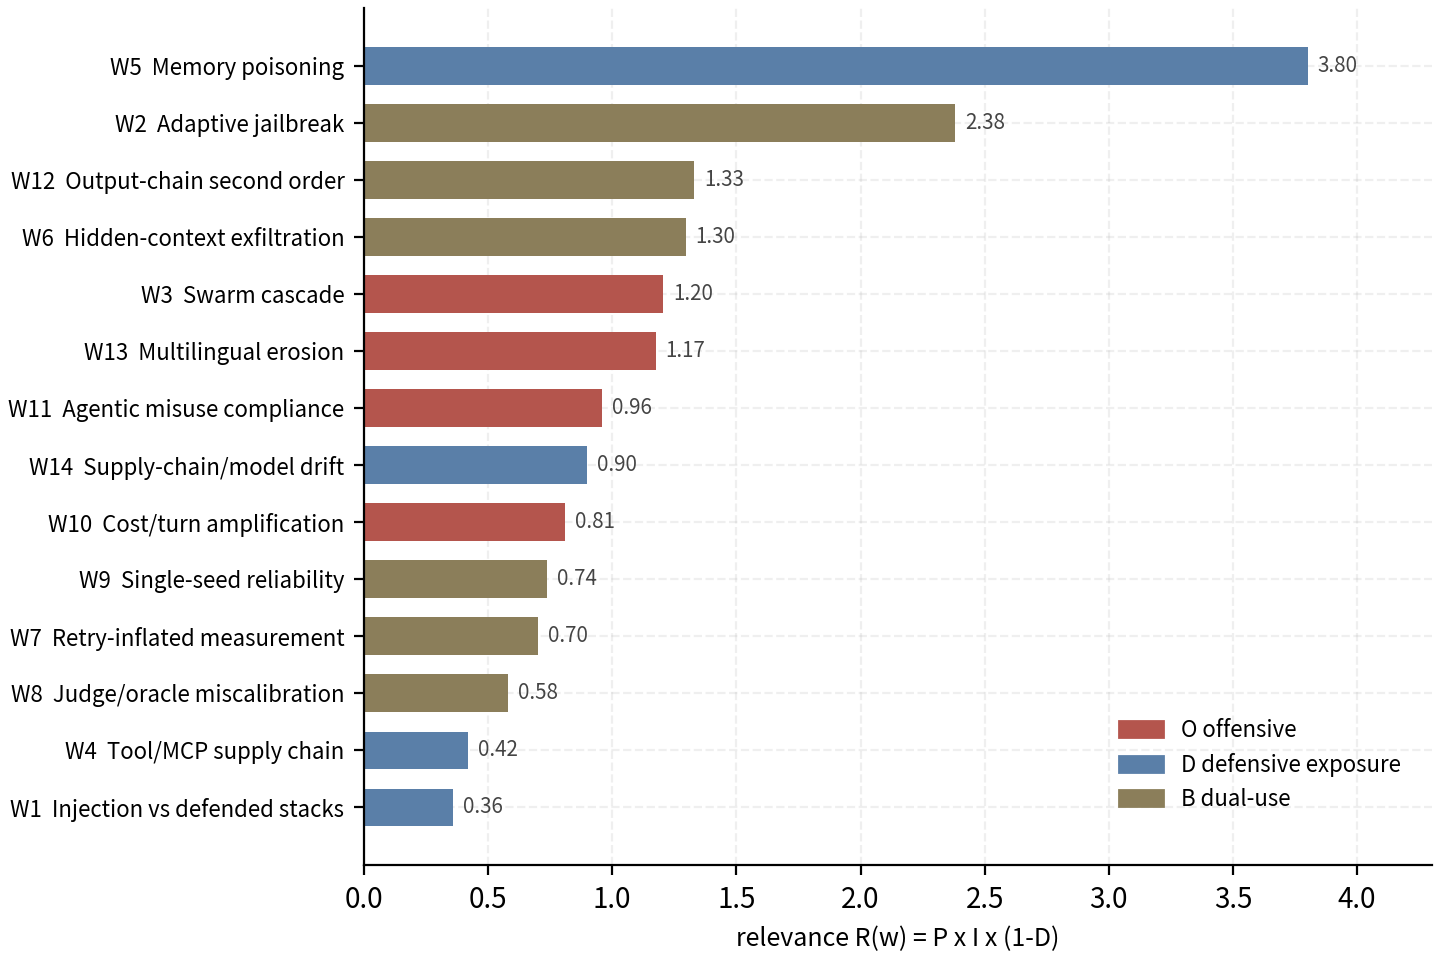
\includegraphics[width=0.94\columnwidth]{fig_relevance.png}
\caption{Relevance ranking $R(w)=P\cdot I\cdot(1-D)$ for W1--W14. Colors: lens
(O offensive, D defensive exposure of our stack, B dual-use). W5 leads because
impact-5 meets near-zero current defenses on a cross-run persistence channel;
W1 is last because a deployed guard stack covers it best---low relevance is
the reward for engineering, not evidence of safety.}\label{fig:relevance}
\end{figure}

\subsection{Probe allocation: bandits, Bayesian optimization, tails}\label{sec:allocation}

Given a probe budget $B$ across attempts with unknown success probabilities, the
allocation problem is a bandit: Thompson sampling (draw each arm's rate from its
posterior, play the argmax) is the standard robust choice, and Bayesian
optimization over structured probe spaces (BRT-style surrogate-guided search)
applies when attempts are expensive \cite{sivakumar-anderson}. Importance-sampling
tail estimation covers the regime that matters most for defenses---the rare
but catastrophic probe---by reweighting cheap attempts toward the tail.
Our framework already runs Thompson sampling over technique selection with
EPSS/KEV warm-started priors \cite{epss-first}; the statistical layer's pooling
machinery is what those posteriors should consume going forward. The paper's
honest position: the statistical layer is ahead of the evaluation layer ---
the estimators exist; wiring every cell card to them is recommendation~8's
first item.
